\documentclass[tikz,border=8pt]{standalone}
\usepackage{tikz}
\usetikzlibrary{calc,positioning,arrows.meta}
\usepackage[T1]{fontenc}
\usepackage[utf8]{inputenc}
\usepackage{amsmath}
%% Paleta
\definecolor{CU}{RGB}{27,38,49}
\definecolor{CNU}{RGB}{238,241,245}
\definecolor{CBRD}{RGB}{200,205,208}
\definecolor{CNEW}{RGB}{192,57,43}
\definecolor{CMO}{RGB}{36,113,163}
\definecolor{CCTR}{RGB}{211,84,0}
\definecolor{CHIT}{RGB}{29,106,57}
\definecolor{CFAL}{RGB}{183,119,13}
\definecolor{CMIS}{RGB}{21,67,96}
\definecolor{CPU}{RGB}{113,125,126}
\begin{document}

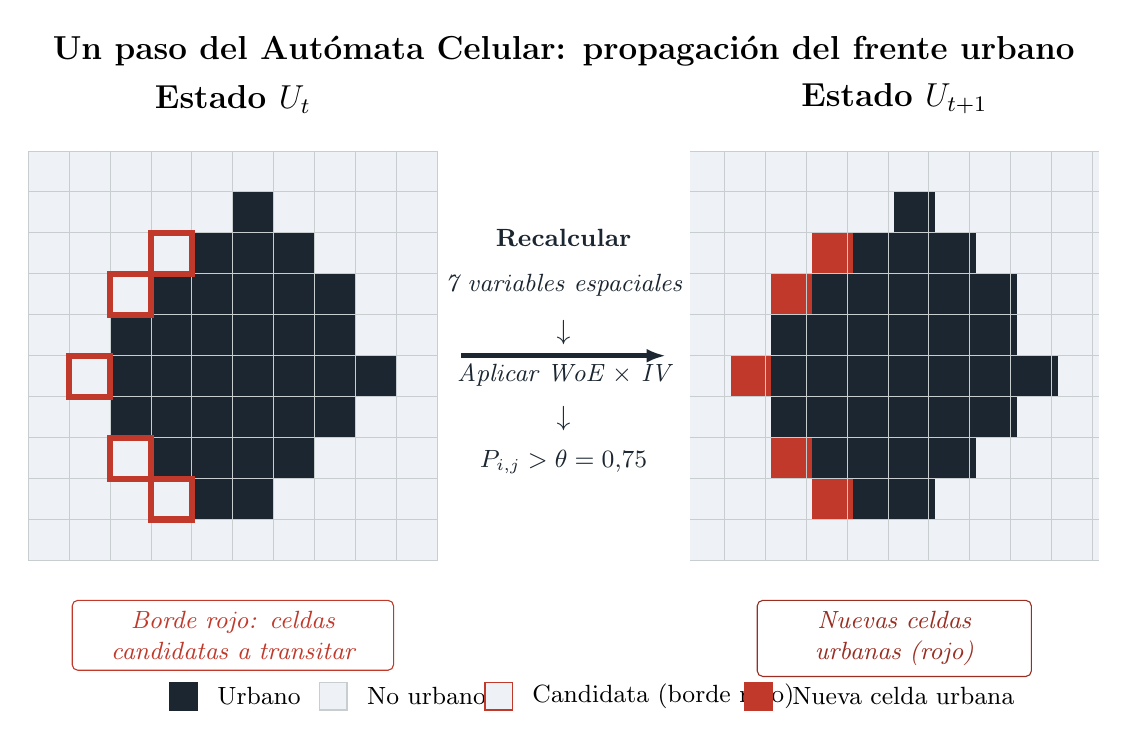
\begin{tikzpicture}[font=\sffamily]
  % — grid background
  \fill[CNU] (0.0000cm,0.0000cm) rectangle (5.2000cm,5.2000cm);
  \fill[CU] (2.6000cm,4.1600cm) rectangle (3.1200cm,4.6800cm);
  \fill[CU] (2.0800cm,3.6400cm) rectangle (2.6000cm,4.1600cm);
  \fill[CU] (2.6000cm,3.6400cm) rectangle (3.1200cm,4.1600cm);
  \fill[CU] (3.1200cm,3.6400cm) rectangle (3.6400cm,4.1600cm);
  \fill[CU] (1.5600cm,3.1200cm) rectangle (2.0800cm,3.6400cm);
  \fill[CU] (2.0800cm,3.1200cm) rectangle (2.6000cm,3.6400cm);
  \fill[CU] (2.6000cm,3.1200cm) rectangle (3.1200cm,3.6400cm);
  \fill[CU] (3.1200cm,3.1200cm) rectangle (3.6400cm,3.6400cm);
  \fill[CU] (3.6400cm,3.1200cm) rectangle (4.1600cm,3.6400cm);
  \fill[CU] (1.0400cm,2.6000cm) rectangle (1.5600cm,3.1200cm);
  \fill[CU] (1.5600cm,2.6000cm) rectangle (2.0800cm,3.1200cm);
  \fill[CU] (2.0800cm,2.6000cm) rectangle (2.6000cm,3.1200cm);
  \fill[CU] (2.6000cm,2.6000cm) rectangle (3.1200cm,3.1200cm);
  \fill[CU] (3.1200cm,2.6000cm) rectangle (3.6400cm,3.1200cm);
  \fill[CU] (3.6400cm,2.6000cm) rectangle (4.1600cm,3.1200cm);
  \fill[CU] (1.0400cm,2.0800cm) rectangle (1.5600cm,2.6000cm);
  \fill[CU] (1.5600cm,2.0800cm) rectangle (2.0800cm,2.6000cm);
  \fill[CU] (2.0800cm,2.0800cm) rectangle (2.6000cm,2.6000cm);
  \fill[CU] (2.6000cm,2.0800cm) rectangle (3.1200cm,2.6000cm);
  \fill[CU] (3.1200cm,2.0800cm) rectangle (3.6400cm,2.6000cm);
  \fill[CU] (3.6400cm,2.0800cm) rectangle (4.1600cm,2.6000cm);
  \fill[CU] (4.1600cm,2.0800cm) rectangle (4.6800cm,2.6000cm);
  \fill[CU] (1.0400cm,1.5600cm) rectangle (1.5600cm,2.0800cm);
  \fill[CU] (1.5600cm,1.5600cm) rectangle (2.0800cm,2.0800cm);
  \fill[CU] (2.0800cm,1.5600cm) rectangle (2.6000cm,2.0800cm);
  \fill[CU] (2.6000cm,1.5600cm) rectangle (3.1200cm,2.0800cm);
  \fill[CU] (3.1200cm,1.5600cm) rectangle (3.6400cm,2.0800cm);
  \fill[CU] (3.6400cm,1.5600cm) rectangle (4.1600cm,2.0800cm);
  \fill[CU] (1.5600cm,1.0400cm) rectangle (2.0800cm,1.5600cm);
  \fill[CU] (2.0800cm,1.0400cm) rectangle (2.6000cm,1.5600cm);
  \fill[CU] (2.6000cm,1.0400cm) rectangle (3.1200cm,1.5600cm);
  \fill[CU] (3.1200cm,1.0400cm) rectangle (3.6400cm,1.5600cm);
  \fill[CU] (2.0800cm,0.5200cm) rectangle (2.6000cm,1.0400cm);
  \fill[CU] (2.6000cm,0.5200cm) rectangle (3.1200cm,1.0400cm);
  \draw[CBRD,line width=0.35pt,xstep=0.5200cm,ystep=0.5200cm] (0.0000cm,0.0000cm) grid (5.2000cm,5.2000cm);
  \draw[CNEW,line width=2.2pt] (1.5600cm,0.5200cm) rectangle (2.0800cm,1.0400cm);
  \draw[CNEW,line width=2.2pt] (1.5600cm,3.6400cm) rectangle (2.0800cm,4.1600cm);
  \draw[CNEW,line width=2.2pt] (0.5200cm,2.0800cm) rectangle (1.0400cm,2.6000cm);
  \draw[CNEW,line width=2.2pt] (1.0400cm,3.1200cm) rectangle (1.5600cm,3.6400cm);
  \draw[CNEW,line width=2.2pt] (1.0400cm,1.0400cm) rectangle (1.5600cm,1.5600cm);
  % — grid background
  \fill[CNU] (8.4000cm,0.0000cm) rectangle (13.6000cm,5.2000cm);
  \fill[CU] (11.0000cm,4.1600cm) rectangle (11.5200cm,4.6800cm);
  \fill[CU] (10.4800cm,3.6400cm) rectangle (11.0000cm,4.1600cm);
  \fill[CU] (11.0000cm,3.6400cm) rectangle (11.5200cm,4.1600cm);
  \fill[CU] (11.5200cm,3.6400cm) rectangle (12.0400cm,4.1600cm);
  \fill[CU] (9.9600cm,3.1200cm) rectangle (10.4800cm,3.6400cm);
  \fill[CU] (10.4800cm,3.1200cm) rectangle (11.0000cm,3.6400cm);
  \fill[CU] (11.0000cm,3.1200cm) rectangle (11.5200cm,3.6400cm);
  \fill[CU] (11.5200cm,3.1200cm) rectangle (12.0400cm,3.6400cm);
  \fill[CU] (12.0400cm,3.1200cm) rectangle (12.5600cm,3.6400cm);
  \fill[CU] (9.4400cm,2.6000cm) rectangle (9.9600cm,3.1200cm);
  \fill[CU] (9.9600cm,2.6000cm) rectangle (10.4800cm,3.1200cm);
  \fill[CU] (10.4800cm,2.6000cm) rectangle (11.0000cm,3.1200cm);
  \fill[CU] (11.0000cm,2.6000cm) rectangle (11.5200cm,3.1200cm);
  \fill[CU] (11.5200cm,2.6000cm) rectangle (12.0400cm,3.1200cm);
  \fill[CU] (12.0400cm,2.6000cm) rectangle (12.5600cm,3.1200cm);
  \fill[CU] (9.4400cm,2.0800cm) rectangle (9.9600cm,2.6000cm);
  \fill[CU] (9.9600cm,2.0800cm) rectangle (10.4800cm,2.6000cm);
  \fill[CU] (10.4800cm,2.0800cm) rectangle (11.0000cm,2.6000cm);
  \fill[CU] (11.0000cm,2.0800cm) rectangle (11.5200cm,2.6000cm);
  \fill[CU] (11.5200cm,2.0800cm) rectangle (12.0400cm,2.6000cm);
  \fill[CU] (12.0400cm,2.0800cm) rectangle (12.5600cm,2.6000cm);
  \fill[CU] (12.5600cm,2.0800cm) rectangle (13.0800cm,2.6000cm);
  \fill[CU] (9.4400cm,1.5600cm) rectangle (9.9600cm,2.0800cm);
  \fill[CU] (9.9600cm,1.5600cm) rectangle (10.4800cm,2.0800cm);
  \fill[CU] (10.4800cm,1.5600cm) rectangle (11.0000cm,2.0800cm);
  \fill[CU] (11.0000cm,1.5600cm) rectangle (11.5200cm,2.0800cm);
  \fill[CU] (11.5200cm,1.5600cm) rectangle (12.0400cm,2.0800cm);
  \fill[CU] (12.0400cm,1.5600cm) rectangle (12.5600cm,2.0800cm);
  \fill[CU] (9.9600cm,1.0400cm) rectangle (10.4800cm,1.5600cm);
  \fill[CU] (10.4800cm,1.0400cm) rectangle (11.0000cm,1.5600cm);
  \fill[CU] (11.0000cm,1.0400cm) rectangle (11.5200cm,1.5600cm);
  \fill[CU] (11.5200cm,1.0400cm) rectangle (12.0400cm,1.5600cm);
  \fill[CU] (10.4800cm,0.5200cm) rectangle (11.0000cm,1.0400cm);
  \fill[CU] (11.0000cm,0.5200cm) rectangle (11.5200cm,1.0400cm);
  \fill[CNEW] (9.9600cm,0.5200cm) rectangle (10.4800cm,1.0400cm);
  \fill[CNEW] (9.9600cm,3.6400cm) rectangle (10.4800cm,4.1600cm);
  \fill[CNEW] (8.9200cm,2.0800cm) rectangle (9.4400cm,2.6000cm);
  \fill[CNEW] (9.4400cm,3.1200cm) rectangle (9.9600cm,3.6400cm);
  \fill[CNEW] (9.4400cm,1.0400cm) rectangle (9.9600cm,1.5600cm);
  \draw[CBRD,line width=0.35pt,xstep=0.5200cm,ystep=0.5200cm] (8.4000cm,0.0000cm) grid (13.6000cm,5.2000cm);
  \draw[-{Latex[length=7pt,width=5pt]},line width=1.8pt,CU] (5.5000cm,2.6000cm) -- (8.1000cm,2.6000cm);
  \node[font=\small,text=CU,align=center] at (6.8000cm,4.1000cm) {\textbf{Recalcular}};
  \node[font=\small\itshape,text=CU,align=center] at (6.8000cm,3.5000cm) {7 variables espaciales};
  \node[font=\normalsize,text=CU,align=center] at (6.8000cm,2.9000cm) {$\downarrow$};
  \node[font=\small\itshape,text=CU,align=center] at (6.8000cm,2.3500cm) {Aplicar WoE $\times$ IV};
  \node[font=\normalsize,text=CU,align=center] at (6.8000cm,1.8000cm) {$\downarrow$};
  \node[font=\small,text=CU,align=center] at (6.8000cm,1.2500cm) {$P_{i,j}>\theta=0{,}75$};
  \node[font=\large\bfseries,anchor=south] at (2.6000cm,5.5500cm) {Estado $U_t$};
  \node[font=\large\bfseries,anchor=south] at (11.0000cm,5.5500cm) {Estado $U_{t+1}$};
  \node[font=\large\bfseries,anchor=south] at (6.8000cm,6.1500cm) {Un paso del Aut\'{o}mata Celular: propagaci\'{o}n del frente urbano};
  \node[draw=CNEW,fill=white,rounded corners=2pt,  text=CNEW,font=\small\itshape,  text width=3.8cm,align=center,inner sep=4pt,  anchor=north] at (2.6000cm,-0.5000cm) {Borde rojo: celdas candidatas a transitar};
  \node[draw=CNEW!80!black,fill=white,rounded corners=2pt,  text=CNEW!80!black,font=\small\itshape,  text width=3.2cm,align=center,inner sep=4pt,  anchor=north] at (11.0000cm,-0.5000cm) {Nuevas celdas urbanas (rojo)};
  \fill[CU] (1.8000cm,-1.9000cm) rectangle (2.1500cm,-1.5500cm);
  \draw[CU,line width=0.6pt] (1.8000cm,-1.9000cm) rectangle (2.1500cm,-1.5500cm);
  \node[font=\small,anchor=west] at (2.2800cm,-1.7250cm) {Urbano};
  \fill[CNU] (3.7000cm,-1.9000cm) rectangle (4.0500cm,-1.5500cm);
  \draw[CBRD,line width=0.6pt] (3.7000cm,-1.9000cm) rectangle (4.0500cm,-1.5500cm);
  \node[font=\small,anchor=west] at (4.1800cm,-1.7250cm) {No urbano};
  \fill[CNU] (5.8000cm,-1.9000cm) rectangle (6.1500cm,-1.5500cm);
  \draw[CNEW,line width=0.6pt] (5.8000cm,-1.9000cm) rectangle (6.1500cm,-1.5500cm);
  \node[font=\small,anchor=west] at (6.2800cm,-1.7250cm) {Candidata (borde rojo)};
  \fill[CNEW] (9.1000cm,-1.9000cm) rectangle (9.4500cm,-1.5500cm);
  \draw[CNEW,line width=0.6pt] (9.1000cm,-1.9000cm) rectangle (9.4500cm,-1.5500cm);
  \node[font=\small,anchor=west] at (9.5800cm,-1.7250cm) {Nueva celda urbana};
\end{tikzpicture}
\end{document}
